\documentclass[10pt,a4paper,twoside,twocolumn]{article}
%% Lots of packages !
\usepackage{etex}

%% Francisation
\usepackage[english]{babel}
\usepackage[T1]{fontenc}
\usepackage[utf8]{inputenc}
%\usepackage{textcomp}

%% Réglages généraux
\usepackage[left=1.5cm,right=1.5cm,top=2cm,bottom=2cm]{geometry}
\usepackage{fancyhdr}
\usepackage{setspace}
\usepackage{lscape}
%\usepackage{multicol}
\usepackage{makeidx}
\usepackage[clearempty]{titlesec}
\usepackage{cite}

%% Packages pour le texte
\usepackage{pifont}
\usepackage{eurosym}
\usepackage{soul}
\usepackage[normalem]{ulem}
\usepackage{fancybox}
\usepackage{boxedminipage}
\usepackage{enumerate}
\usepackage{verbatim}
\usepackage{moreverb}
\usepackage{listings}
\usepackage[table]{xcolor}

%% Packages pour les tableaux
\usepackage{array}
\usepackage{multirow}
\usepackage{tabularx}
\usepackage{longtable}

%% Packages pour les dessins
\usepackage{graphicx}
\usepackage{wrapfig}
%\usepackage{picins}
\usepackage{picinpar}
\usepackage{epic}
\usepackage{eepic}
\usepackage{tikz}
\usepackage{afterpage}
\usepackage{rotating}
\usepackage{float}
\usepackage{caption}

%% Packages pour les maths
\usepackage{amsmath}
\usepackage{amssymb}
\usepackage{dsfont}
\usepackage{mathrsfs}
\usepackage{bussproofs}
\usepackage[thmmarks,amsmath]{ntheorem}

%% Création de nouvelles commandes
%\usepackage{calc}
\usepackage{ifthen}
\usepackage{xspace}



\usepackage{url}
\usepackage{hyperref}
\usepackage{todonotes}
\usepackage{subcaption}
\usepackage[french,ruled,vlined,linesnumbered,algosection,dotocloa]{algorithm2e}
\usepackage{MnSymbol}

\usepackage{chngcntr}

\usepackage{standalone}
\usepackage{import}

\usepackage[affil-it]{authblk}


\usepackage{lipsum}












\numberwithin{equation}{subsection}


\newcommand*{\rootPath}{../}
\standalonetrue

\begin{document}

\section{Results}

\subsection{Single error injection}

Our single bit flip experiment had expected yet interresting results.

Injecting a single bit flip moves on particle by modifiying one of its floating
coordinates. While some bit's position only have a small impact, other can have
an impact on the pipeline. Modification of the exponent bits can make the
affected particule exit the donsidered domain, which some code cannot handle.
As a consequensed, some bit flips cause Tess-Dense to crash. Other code, like
our AKDE implementation can handle particle exiting the domain and, for such
corruption in fact produce silent errors.

The first conclusion that some specific memory corruption produce hard errors
due to bad coding practices. Those same memory corruption can in fact be
detected inside the process by checking that the data verify some specific
criterion.

Once the corrupted sampling processed using AKDE, the resulting density could
not be distinguish for expected results ass they where whitin the range of
expected results. This was to be expected has a single memory corruption could
be seen as a verry slight modification of one of many particles in the
intrinsically random sampling and therefore be statically indiscernible.

\subsection{Multiple error injection}

Figure~\ref{fig:bitflip-fields} shows the density field computed by AKDE after
injection of random bit flips.

\begin{figure*}[!ht]
	\centering
	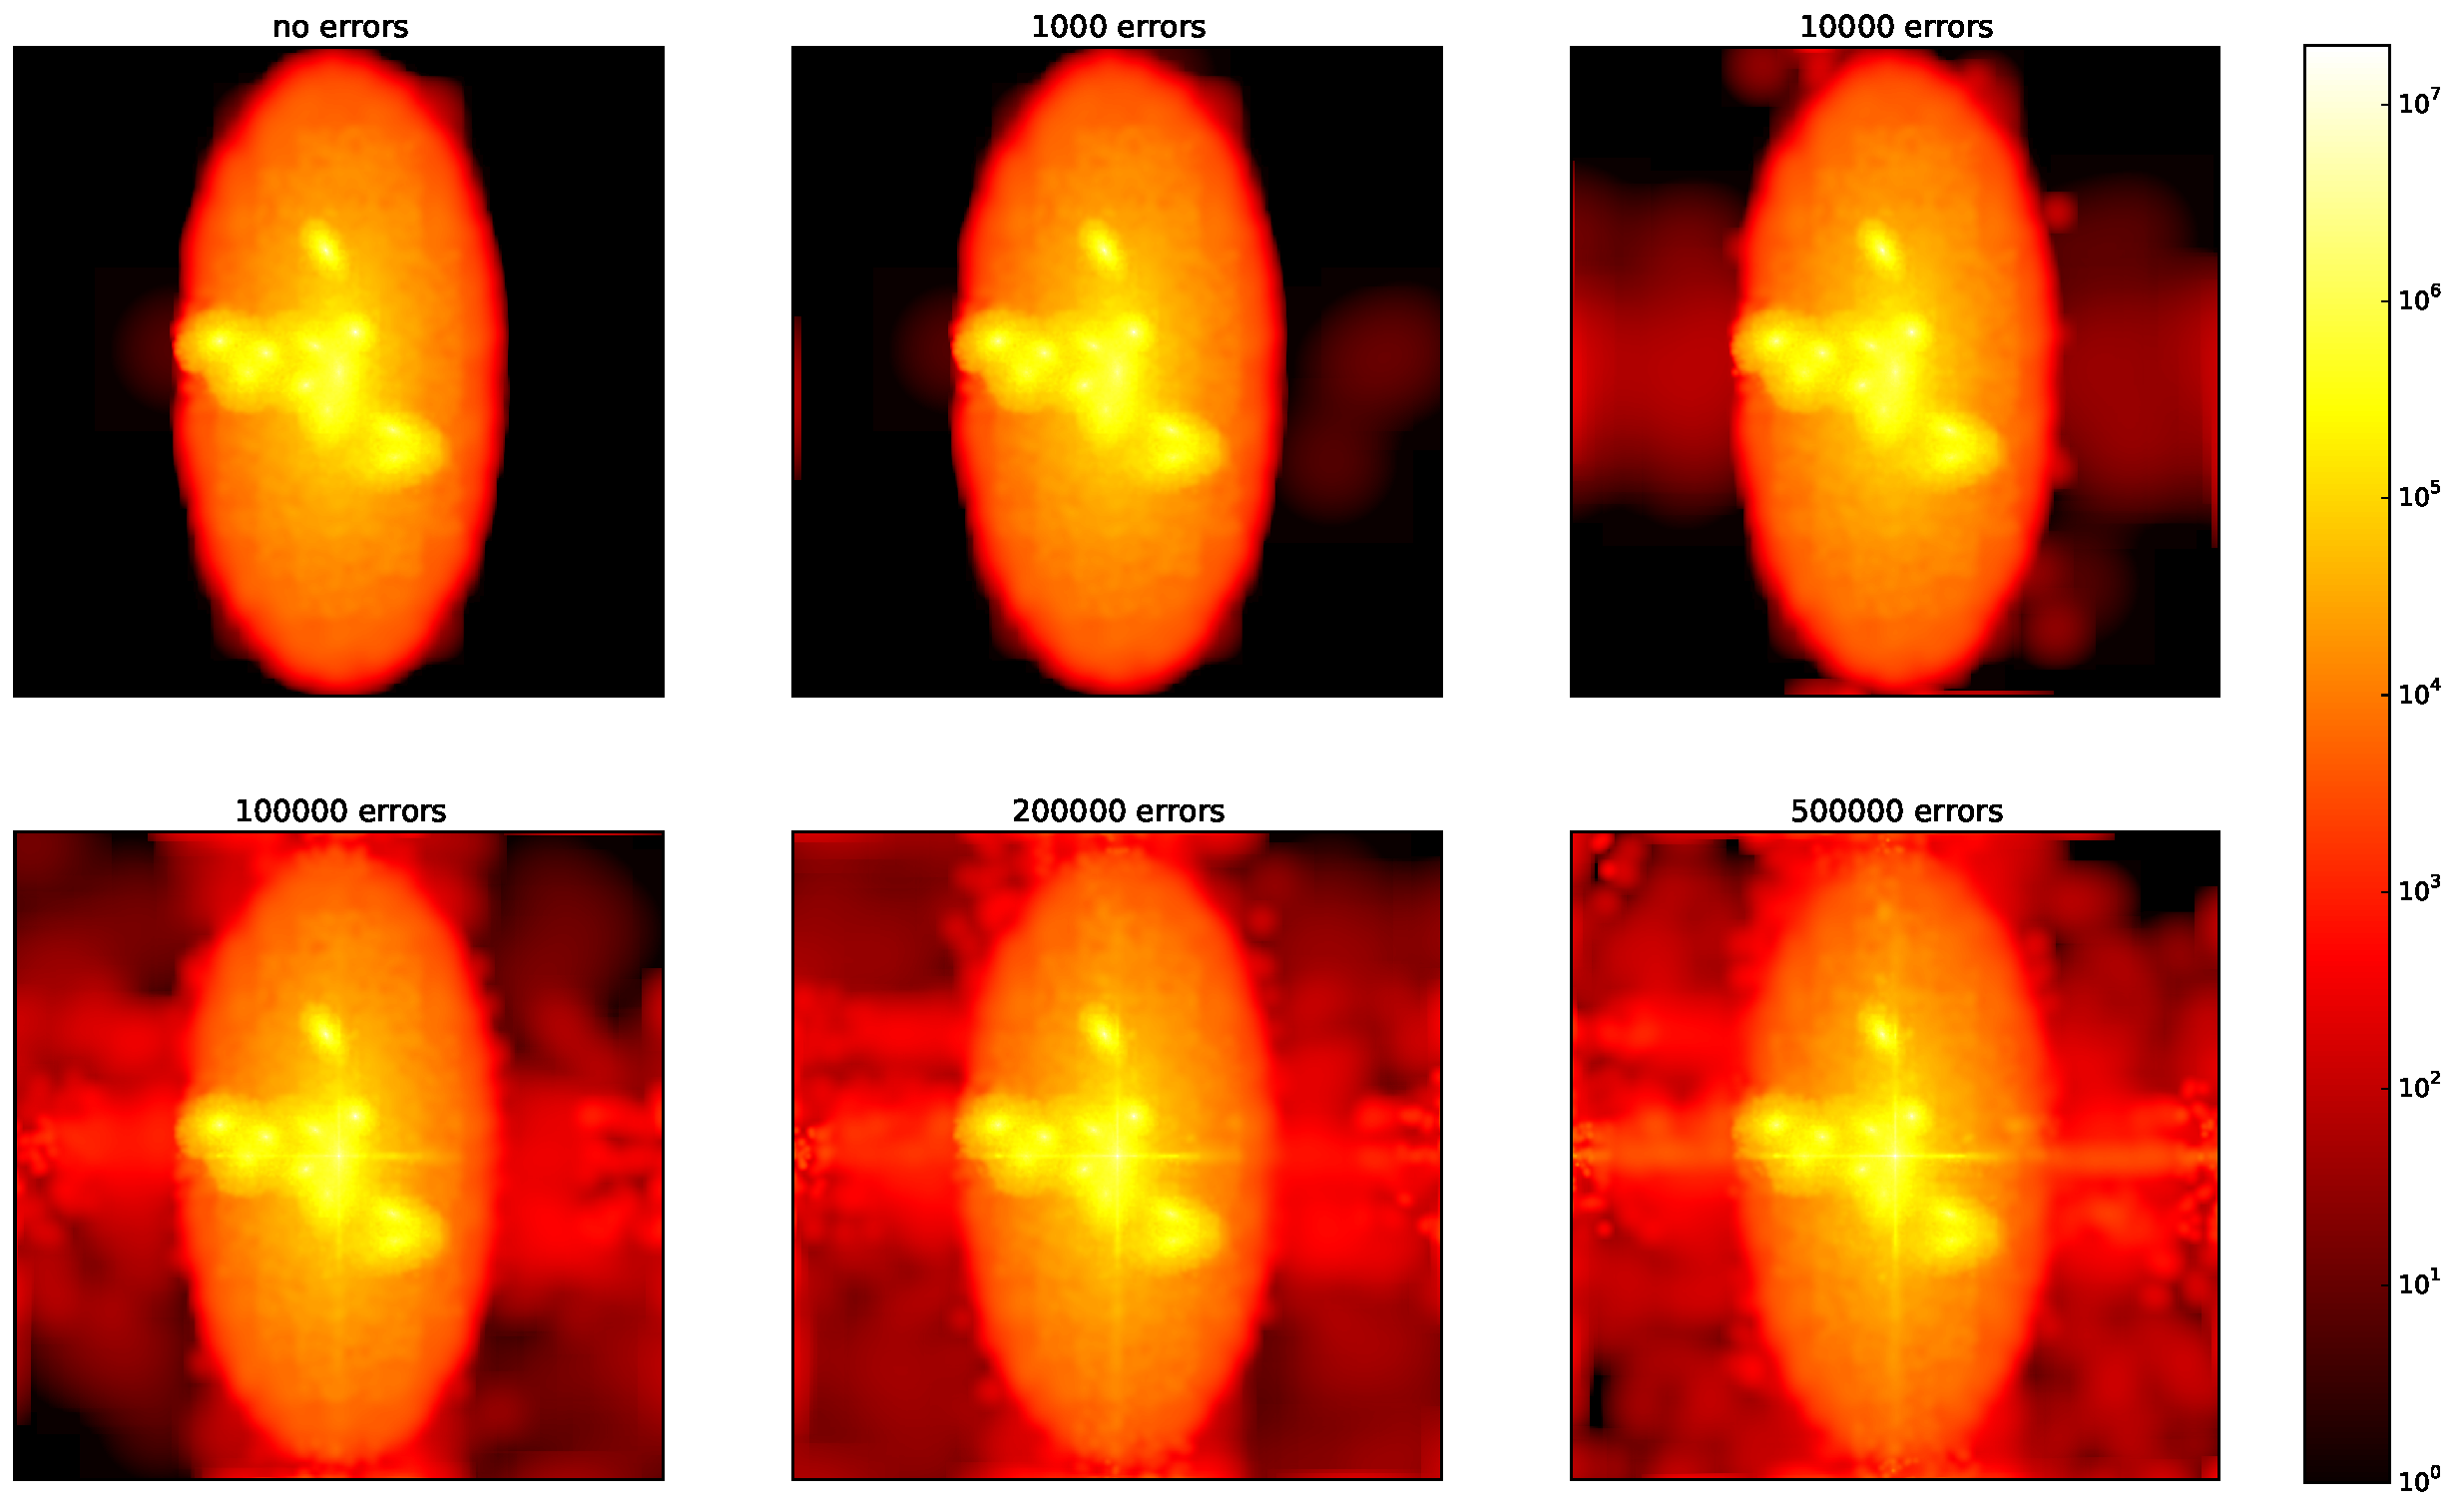
\includegraphics[width=0.9\textwidth]
		{\rootPath Figures/randomized-multiplot.pdf}
	\caption{AKDE density fields after error injection}
	\label{fig:bitflip-fields}
\end{figure*}

Beyound the small noise on the sides, made visible by the density log scale, an
cross is visible at the center of the domain. This cross is caused by bit flips
in exponent part of floating point values, making them converge toward $0$. We
therefore have a high density around plane $\mathcal P_{x=0}$,
$\mathcal  P_{y=0}$ and $\mathcal P_{z=0}$.

Figure~\ref{fig:bitflip-spectral} shows the power spectrum of those density
fields.

\begin{figure*}[!ht]
	\centering
	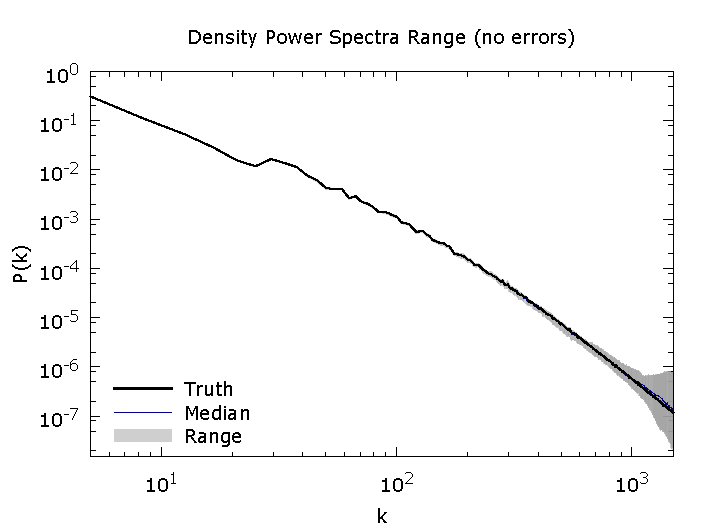
\includegraphics[width=0.32\textwidth]
		{\rootPath Figures/cnfw_err/cnfw_particles_2e5_akde_err0_clamped.pdf}
	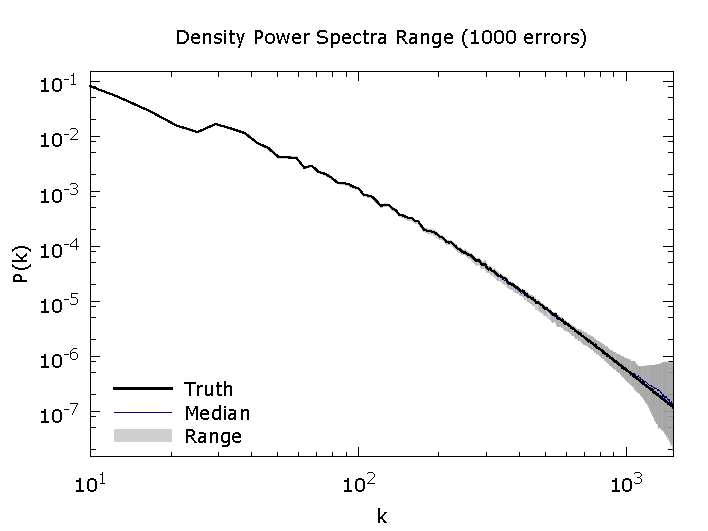
\includegraphics[width=0.32\textwidth]
		{\rootPath Figures/cnfw_err/cnfw_particles_2e5_akde_err1000_clamped.pdf}
	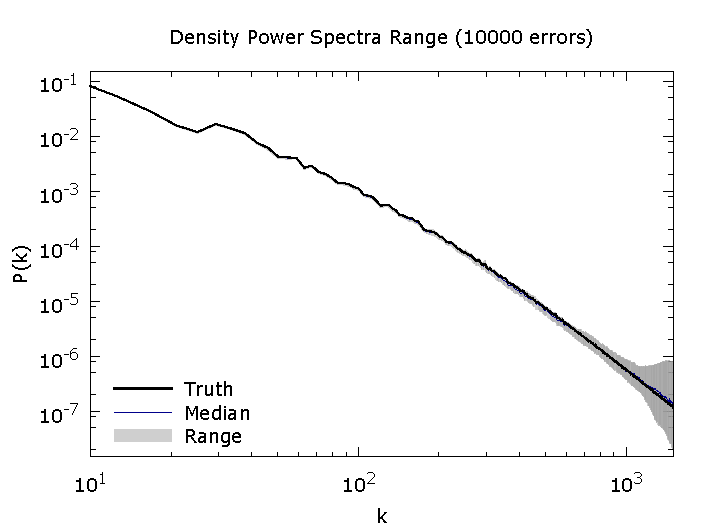
\includegraphics[width=0.32\textwidth]
		{\rootPath Figures/cnfw_err/cnfw_particles_2e5_akde_err10000_clamped.pdf}
	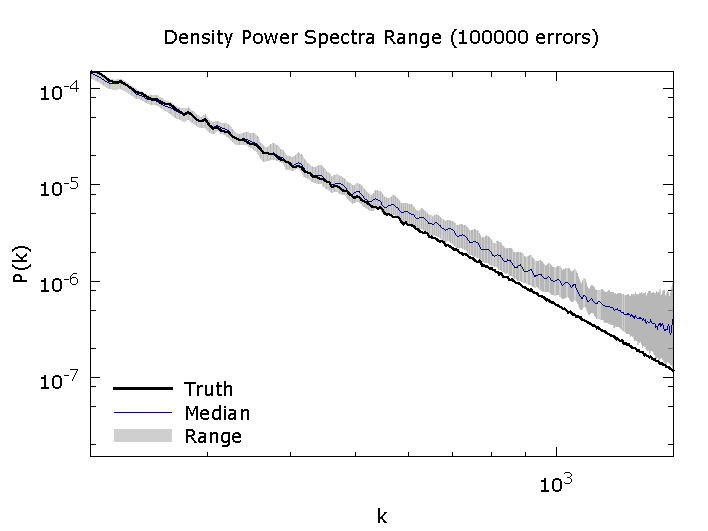
\includegraphics[width=0.32\textwidth]
		{\rootPath Figures/cnfw_err/cnfw_particles_2e5_akde_err100000_clamped.pdf}
	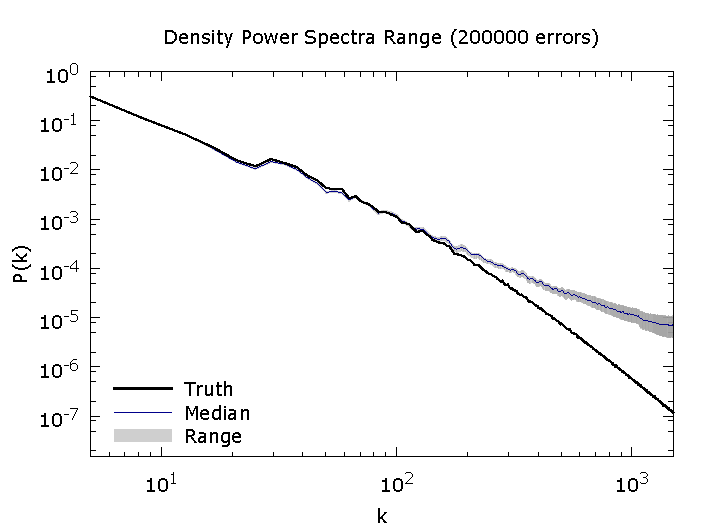
\includegraphics[width=0.32\textwidth]
		{\rootPath Figures/cnfw_err/cnfw_particles_2e5_akde_err200000_clamped.pdf}
	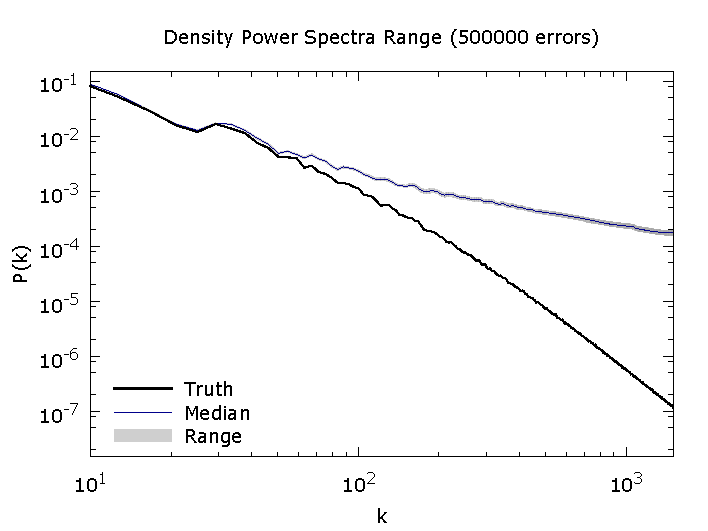
\includegraphics[width=0.32\textwidth]
		{\rootPath Figures/cnfw_err/cnfw_particles_2e5_akde_err500000_clamped.pdf}
	\caption{Bitflip influence on AKDE power spectrum range}
	\label{fig:bitflip-spectral}
\end{figure*}

Those results both show a discrepancy between corrupted pipeline and expected 
results for error numbers between $10^4$ and $10^5$. Considering the size of our
input, that represent a corruption probability of $10^{-4}$.



\begin{figure}[!ht]
	\centering
	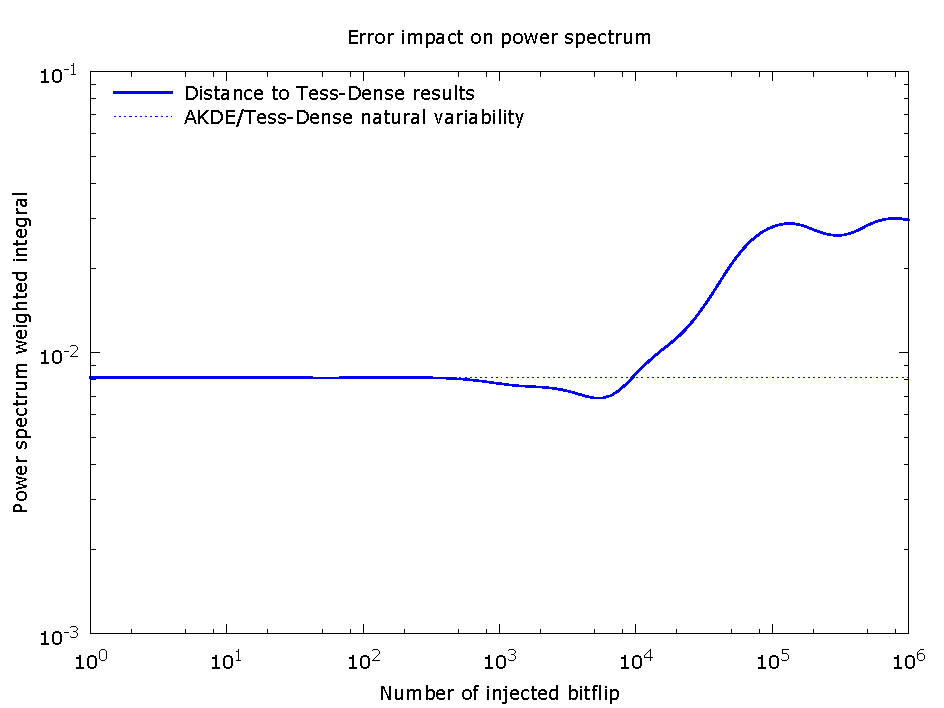
\includegraphics[width=0.45\textwidth]
		{\rootPath Figures/pk-integral.pdf}
	\caption{Power spectrum displacement}
	\label{fig:bitflip-integral}
\end{figure}

%=====================================================================
%=====================================================================
\ifstandalone
	\bibliographystyle{apalike}
	\bibliography{\rootPath Annexes/biblio}
\fi
%=====================================================================
%=====================================================================
\end{document}
